\setcounter{ExampleCounter}{1}
Earlier in this chapter, we considered simple loans, but in each case, we assumed that we took out a loan at one point, let interest accrue, and paid back a lump sum later.  However, many loans are \textbf{installment loans} (or \textbf{amortized loans}), where the loan principal is paid back in smaller regular payments over time, ultimately bringing the balance to zero.  Most common loans, like mortgages, car loans, and student loans, are installment loans.

To see how installment loans work, consider this example: suppose you borrow \$5000 and need to pay it off in 5 years, with 8\% annual interest.  There are many ways to pay off a loan, but let's investigate three in particular:
\begin{itemize}
\item Plan 1 is to pay the principal and interest all together in a single payment at the end of five years.
\item Plan 2 is to pay each year's interest at the end of that year, then pay the principal at the end of the last year.
\item Plan 3 is to pay in five equal end-of-year payments.
\end{itemize}
The following table compares the three plans (note especially the total payment for each plan).
\begin{center}
\begin{tabular}{c *5{>{\raggedright\arraybackslash}p{0.7in}} p{1in} p{1in} p{1in} p{1in}}
{\small Year} & {\small\raggedright Owed at Beginning} & {\small Interest Owed} & {\small Total Owed at End} & {\small Principal Payment} & {\small Total Payment}\\
\hline
\multicolumn{6}{l}{\small Plan 1: Pay principal and interest in one payment at end of 5 years}\\
1 & 5000 & 400 & 5400 & 0 & 0\\
2 & 5400 & 432 & 5832 & 0 & 0\\
3 & 5832 & 467 & 6299 & 0 & 0\\
4 & 6299 & 504 & 6803 & 0 & 0\\
5 & 6803 & 544 & 7347 & 5000 & 7347\\
\textbf{Total} & & \textbf{2347} & & \textbf{5000} & \textbf{7347}\\
\hline
\multicolumn{6}{l}{\small Plan 2: Pay interest due at the end of each year and principal at end of 5 years}\\
1 & 5000 & 400 & 5400 & 0 & 400\\
2 & 5000 & 400 & 5400 & 0 & 400\\
3 & 5000 & 400 & 5400 & 0 & 400\\
4 & 5000 & 400 & 5400 & 0 & 400\\
5 & 5000 & 400 & 5400 & 5000 & 5400\\
\textbf{Total} & & \textbf{2000} & & \textbf{5000} & \textbf{7000}\\
\hline
\multicolumn{6}{l}{\small Plan 3: Pay in five equal end-of-year payments}\\
1 & 5000 & 400 & 5400 & 852 & 1252\\
2 & 4148 & 331 & 4479 & 921 & 1252\\
3 & 3227 & 258 & 3485 & 994 & 1252\\
4 & 2233 & 178 & 2411 & 1074 & 1252\\
5 & 1159 & 93 & 1252 & 1159 & 1252\\
\textbf{Total} & & \textbf{1260} & & \textbf{5000} & \textbf{6260}\\
\hline
\end{tabular}
\end{center}

There's a lot going on in this table, but for now, we just want to notice a few things.  First of all, it is clearly to the borrowers advantage to use the third plan, which uses installment payments to pay back the principal and interest, since the borrower ends up paying only \$6260 total.  Next, notice that this was accomplished with equal payments of \$1252, although we don't know just yet how this payment amount was calculated (we'll get to that shortly).  Finally, the third section of the table, which lays out the details of the installment plan, is similar to an \textbf{amortization schedule}, which we'll see later on; it is simply a schedule of each payment, how much interest is due at that point, and how the payments is split between interest and principal.

Notice that as the years go by, the interest owed decreases as the balance is paid off, but the same amount is paid each year.  This means that the amount of the payment that can go toward the principal increases each year as less of it is taken by the interest.  This means that when you purchase a home or a car or start paying off student loans, your early payments will go almost completely toward interest (which can be depressing) and your last payments will go almost completely toward the principal (which is much better).
\pagebreak

\paragraph{Calculating the payment on an installment loan:} Calculating a periodic payment like the one that appeared in the table above is based on what we've already seen regarding annuities; in fact, an installment loan is exactly a payout annuity.\\

To see this, imagine that you had \$5000 invested at a bank and you started taking out payments while earning interest (a payout annuity), and after 5 years your balance was zero.  Now flip that around and put yourself in the position of a bank: now the lender is investing \$5000 in you (you take a loan of \$5000) and you start to pay them back in equal payments as the remaining balance earns interest, and after 5 years the balance is zero.\\

Knowing this, we can simply copy the formula for payout annuities, but this time we'll rearrange the terms to solve for $PMT$, since we'll mostly be interested in calculating the payment amount for an installment loan.\\

\begin{formula}{Installment Loan Payment}
If an installment loan of $P$ is taken out at an interest rate of $r$ compounded $n$ times a year, and paid back in equal payments $n$ times a year over $t$ years, the payment amount $PMT$ is given by
\[PMT = \dfrac{P\left(\dfrac{r}{n}\right)}{1-\left(1+\dfrac{r}{n}\right)^{-nt}}\]
\end{formula}
\vspace{0.5in}

\begin{example}[https://www.youtube.com/watch?v=RVUWTbil3fQ]{Car Loan}
If you take out an auto loan of \$11,000 at 4\% interest for 60 months, what will your monthly payment be?\\

\marginnote{\bfseries Solution}
Organize what's given:
\begin{center}
\begin{tabular}{r l l}
$P$ & \$11,000 & The loan amount\\
$r$ & 0.04 & 4\% interest rate\\
$n$ & 12 & Payments made monthly\\
$t$ & 5 & 60 months = 5 years
\end{tabular}
\end{center}

Simply use the formula:
\begin{align*}
PMT &= \dfrac{\$11,000\left(\dfrac{0.04}{12}\right)}{1-\left(1+\dfrac{0.04}{12}\right)^{-(12)(5)}}\\
&= \$202.58
\end{align*}
Thus you'll end up paying \$202.58 every month for five years.
\end{example}

\begin{try}[http://izzomath.com/103text/finance/example5.1/story.html]
If you take out an auto loan of \$15,000 at 5.6\% interest for 72 months, what will your monthly payment be?
\end{try}

Now let's flip the question around: if you can budget for a car payment, how much of a loan can you afford?
\vfill
\pagebreak

\begin{example}[https://www.youtube.com/watch?v=ydmN5lt5g20]{How Much Can You Afford?}
You can afford a monthly car payment of \$250.  If you find a bank offering 4.85\% interest on a 60 month loan, what is the largest car loan you can afford?\\

\marginnote{\bfseries Solution}
In this case $PMT$ is known and $P$ is the unknown that we want to find:
\begin{center}
\begin{tabular}{r l l}
$PMT$ & \$250 & The loan amount\\
$r$ & 0.0485 & 4.85\% interest rate\\
$n$ & 12 & Payments made monthly\\
$t$ & 5 & 60 months = 5 years
\end{tabular}
\end{center}

Now use the formula and solve for $P$:
\begin{align*}
\$250 &= \dfrac{P\left(\dfrac{0.0485}{12}\right)}{1-\left(1+\dfrac{0.0485}{12}\right)^{-(12)(5)}}\\
\$250 &= P(0.0188)
\$13,296 &= P
\end{align*}
You can afford a car loan of \$13,296 under these terms; of course, this is the maximum you can afford, so it wouldn't hurt to take out a smaller loan that this if you can.
\end{example}

\begin{try}[http://izzomath.com/103text/finance/example5.2/story.html]
You can afford a monthly car payment of \$300.  If you find a bank offering 6.7\% interest on a 48 month loan, what is the largest car loan you can afford?
\end{try}

\begin{example}[https://www.youtube.com/watch?v=rhTeMJm8-Lc]{Actual Cost}
You see a TV ad that says ``We can put you in the car of your dreams!!! Drive this brand-new \$25,000 car off the lot with only \$500 down and a monthly payment of \$550 for 60 months.''  How much do you end up actually paying for the car?\\

\marginnote{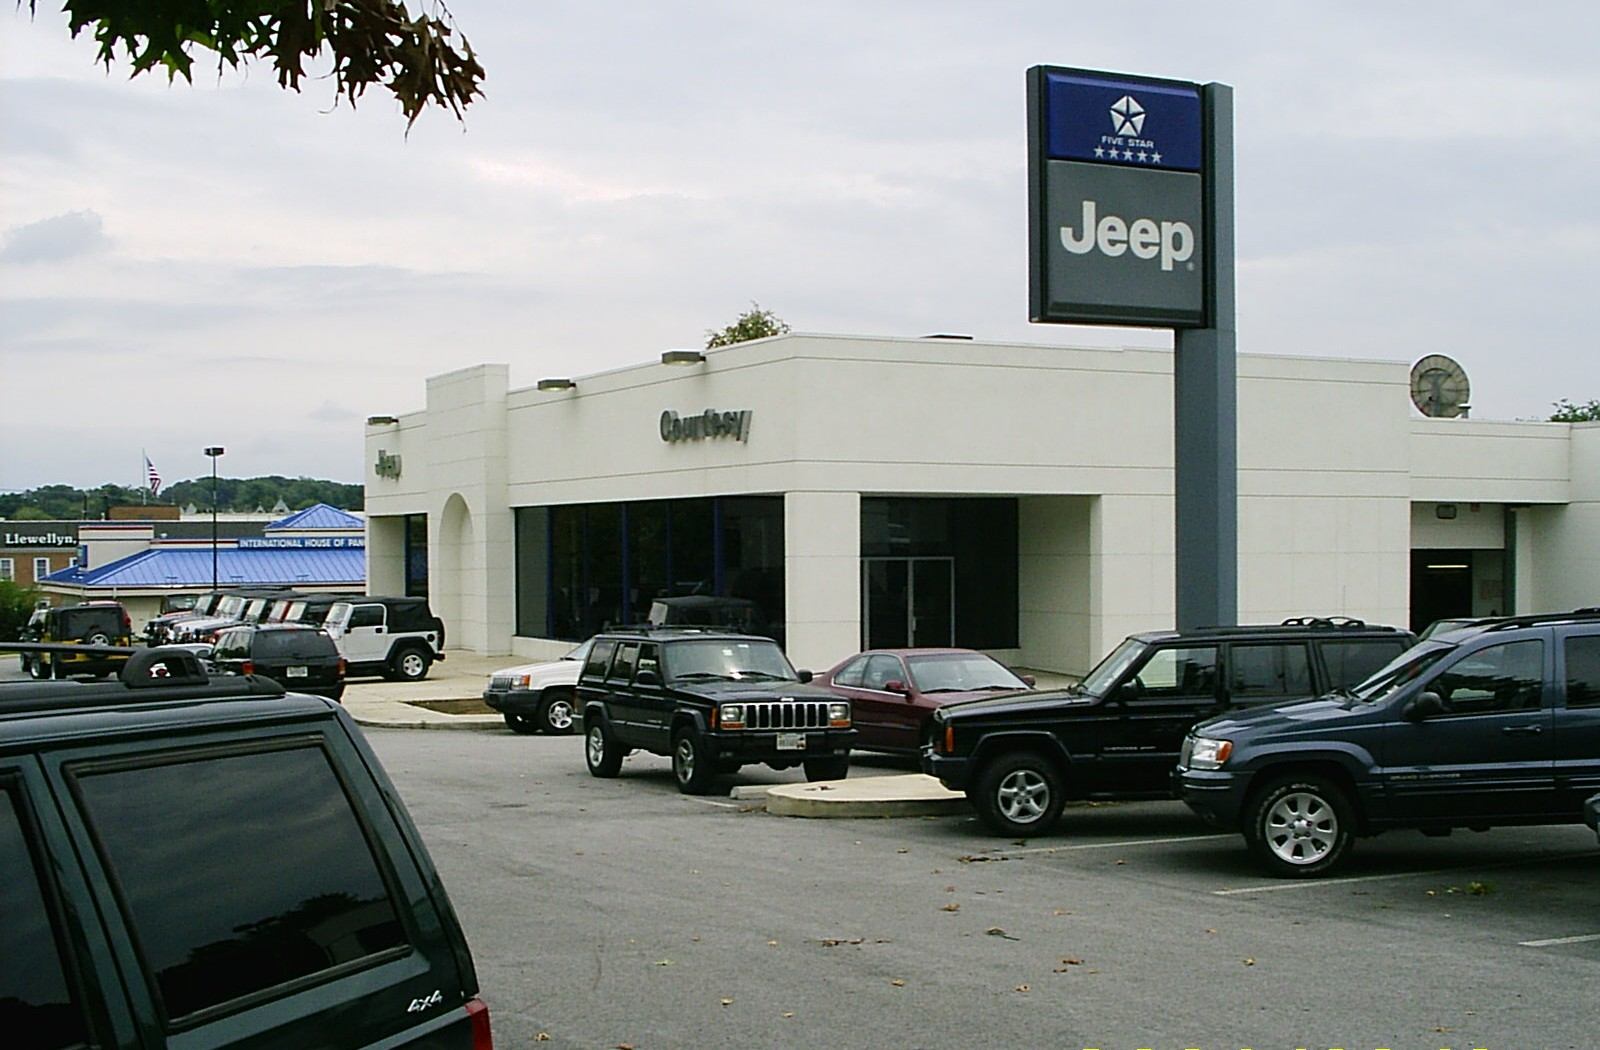
\includegraphics[scale=0.06]{CarDealer1}}
First, let's find out how much the car actually costs you.

The down payment is the amount that is due at the beginning, so if we add that to 60 payments of \$550, we'll have the total amount that comes out of your pocket:
\[\$500 + (60)(\$550) = \$33,500\]

This means that you pay \$33,500 for a \$25,000 car, and the difference is the interest on the loan:\marginnote{\footnotesize\textcolor{black!60}{Photo by Christopher Ziemnowicz}}
\[\$33,500 - \$25,000 = \$8500\]

Are you really willing to pay \$8500 in interest to have the car now, or can you save up first and pay for it in cash---at least in part---to reduce this interest cost?
\end{example}

\begin{try}[http://izzomath.com/103text/finance/example5.3/story.html]
A boat costs \$12,000, and you're offered a loan that requires \$1000 down and \$250 a month for 60 months.  Find the total amount you would pay for the boat and the amount of interest you would pay with this loan.
\end{try}

This example emphasizes an important point: when you're offered a loan, don't focus on the monthly payment; instead, calculate the total cost of the loan and decide if it is worth it to you.
\vfill
\pagebreak

\subsection{Mortgages}
At some point, you'll most likely encounter a \textbf{mortgage}, which is a long-term fixed installment loan, most commonly used to purchase a house.  However, a mortgage is simply a large loan used to purchase property, where the property serves as collateral for the loan.  In case you happen to care, the word ``mortgage'' comes from the Old French \textit{mort} ``dead'' -- \textit{gage} ``pledge.''  The idea of a ``dead pledge'' is that the responsibility dies when the debt is paid off.\\

\marginnote{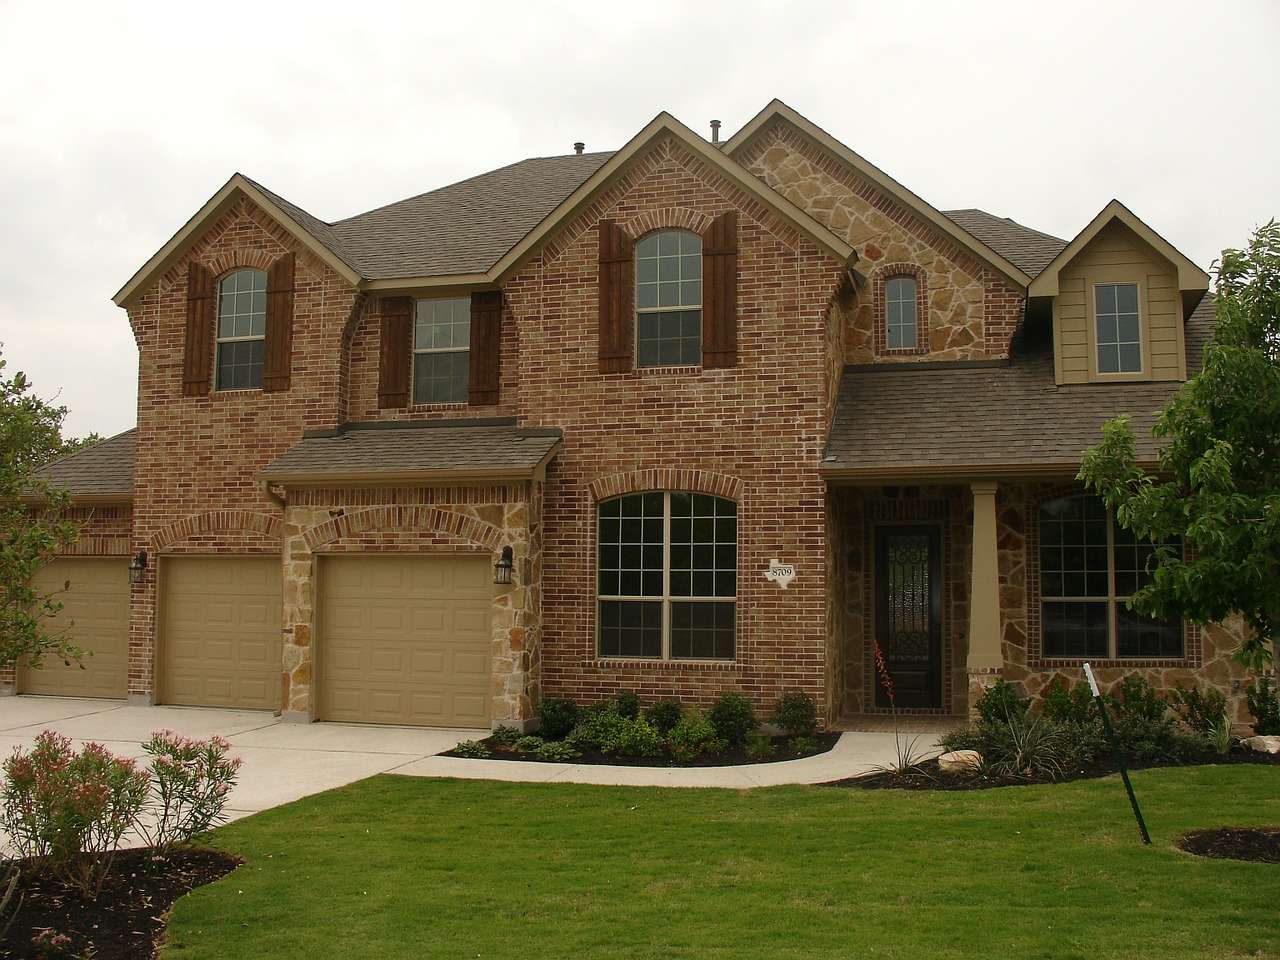
\includegraphics[scale=0.08]{House2}}
We'll focus on mortgages that are used to buy homes in this section, since that is the most practical application.  Most of us don't have the cash to buy a home upfront, so instead we find a bank that is willing to loan us enough to do so.  However, the bank usually isn't willing to loan the entire amount; from their perspective, if a debtor doesn't have anything invested in the loan, they're more likely to \textit{default} on the loan, meaning that they stop making payments and lose the home.  To avoid this, the bank requires a \textbf{down payment}, which means that the buyer is required to come up with a portion of the cost of the home.  The more that the buyer can put down on the home, the less they have to borrow, so they end up paying much less in interest.  Ideally, a buyer is able to put down 20\% of the price of the home; if not, most banks require \textit{mortgage insurance}---which is an extra monthly charge---because clients with less stake in the home are more likely to default, so the bank protects itself with this insurance.

\begin{proc}{Mortgage Terminology}
\begin{itemize}
\item \textbf{Down Payment:} A portion of the cost of the home that the buyer is required to pay before the bank is willing to offer them a loan.
\item \textbf{Loan Amount:} The amount that the bank pays for the home (the cost of the home minus the down payment), which the buyer begins to pay back with monthly payments.
\item \textbf{Closing Costs:} Administrative costs that the bank charges when a mortgage is acquired.  These are usually expressed as \textit{points}, which refers to a percentage of the \textit{loan amount}---not the cost of the home.  Often in negotiations, the seller of the home will agree to cover closing costs in order to make the sale, since the buyer is using all of their available cash to cover the down payment and the seller is the one who will receive a lump sum payment from the bank, so they'll have more cash available.
\end{itemize}
\end{proc}

\begin{example}[https://www.youtube.com/watch?v=lcCuSQxX--Y]{Buying a Condo}
The price of a condominium is \$180,000.  The bank requires a 5\% down payment and one point at closing.  You plan to finance the condominium with a 30-year mortgage at 4\% interest.\\

\begin{center}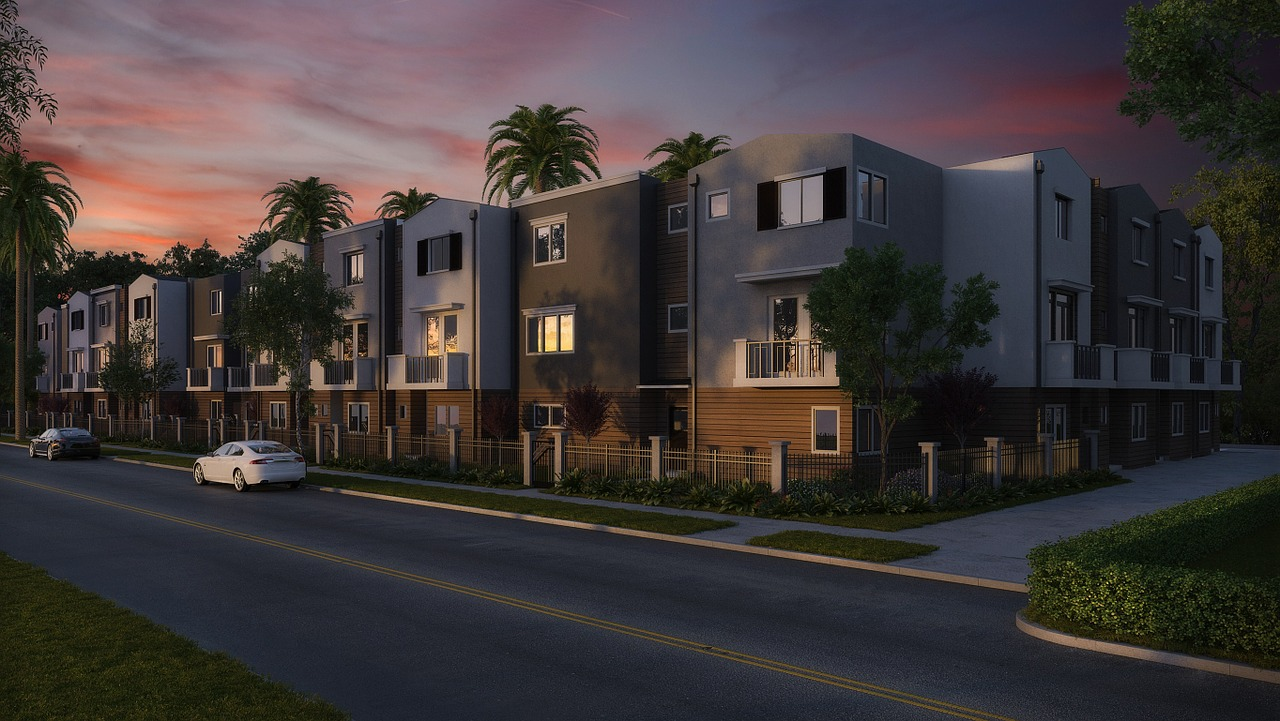
\includegraphics[scale=0.25]{Condo1}\end{center}
\vfill
\pagebreak
\begin{enumerate}[(a)]
\item Find the required down payment.

This is simply 5\% of the sale price, \$180,000:
\[(0.05)(\$180,000) = \$9000\]
Notice that this is the \textit{minimum} down payment; if you were able to put down more than this, that would be a good idea, since it would reduce the interest that you would have to pay in the long run.
\pagebreak

\item Find the loan amount.

This is simply the sale price minus the down payment:
\[\$180,000 - \$9000 = \$171,000\]

\item Find the closing costs.

This will be 1\% of the loan amount, and won't reduce the amount of the loan; it is simply a fee added for the privilege of taking out the loan:
\[(0.01)(\$171,000) = \$1710\]

\item Find the monthly payment.

Here we use the formula for the payment on a fixed installment loan---notice that $n=12$ since this is a monthly payment:
\begin{align*}
PMT &= \dfrac{P\left(\dfrac{r}{n}\right)}{1-\left(1+\dfrac{r}{n}\right)^{-nt}}\\
&= \dfrac{\$171,000\left(\dfrac{0.04}{12}\right)}{1-\left(1+\dfrac{0.04}{12}\right)^{-(12)(30)}}\\
&= \$816.38
\end{align*}

\item Find the total interest paid over 30 years.

Simply find the total amount paid---the down payment plus the 360 monthly payments of \$816.38---and subtract the cost of the condo:
\[\$9000+(360)(\$816.38)-\$180,000 = \$122,896.86\]
Notice that you'll end up paying close to the cost of the condo just in interest.
\end{enumerate}
\end{example}

\begin{try}[http://izzomath.com/103text/finance/example5.4/story.html]
The price of a home is \$340,000.  The bank requires a 10\% down payment and two points at closing.  You plan to finance the condominium with a 30-year mortgage at 3.5\% interest.
\begin{enumerate}[(a)]
\item Find the required down payment.
\item Find the loan amount.
\item Find the closing costs.
\item Find the monthly payment.
\item Find the total interest paid over 30 years.
\end{enumerate}
\end{try}
\pagebreak

\begin{example}[https://www.youtube.com/watch?v=J5Buue07f44]{Comparing Two Mortgages}
The price of a home is \$160,000.  The bank requires a 15\% down payment, and you're offered two mortgage options: 15-year fixed at 5\% or 30-year fixed at 5\% (the term \textit{fixed} here refers to a fixed interest rate, which will be constant throughout the life of the loan, as opposed to an \textit{adjustable-rate mortgage}, or ARM).  Calculate the amount of interest paid for each option and compare the results.\\

\marginnote{\bfseries Solution}
The 15\% down payment will be $(0.15)(\$160,000) = \$24,000$, so the loan amount will be $\$160,000-\$24,000 = \$136,000$.
\begin{enumerate}[(a)]
\item The 15-year mortgage:
\begin{align*}
PMT &= \dfrac{P\left(\dfrac{r}{n}\right)}{1-\left(1+\dfrac{r}{n}\right)^{-nt}}\\
&= \dfrac{\$136,000\left(\dfrac{0.05}{12}\right)}{1-\left(1+\dfrac{0.05}{12}\right)^{-(12)(15)}}\\
&= \$1075.48
\end{align*}

Thus, the amount of interest paid is the monthly payment times 180 (12 payments a year for 15 years) minus the loan amount:
\[(180)(\$1075.48)-\$136,000 = \$57,586.40\]

\item The 30-year mortgage:
\begin{align*}
PMT &= \dfrac{\$136,000\left(\dfrac{0.05}{12}\right)}{1-\left(1+\dfrac{0.05}{12}\right)^{-(12)(30)}}\\
&= \$730.08
\end{align*}

Here there are 360 payments (12 payments a year for 30 years):
\[(360)(\$730.08)-\$136,000 = \$126,828.80\]
\end{enumerate}

If all you see is the monthly payments, the 30-year mortgage is attractive, since the payment is so much lower.  However, over time, you'll pay nearly \$70,000 more in interest simply by stretching the payments over more time.  Now, of course, you may not be able to afford the payments of the 15-year mortgage, so you may be forced to take a longer loan.\\

Because shorter mortgages save so much on interest, banks usually offer lower interest rates on longer mortgages than they do on short ones.
\end{example}
\vfill
\pagebreak

\paragraph{Amortization Schedules}
We've already seen a sort of amortization schedule at the introduction to installment loans with the table that broke down payments one by one.  Here we'll show a more typical layout for an amortization table.

\begin{formula}{Amortization Table}
An \textbf{amortization table} simply lists the payments of an installment loan in order, showing the amount of each payment that goes toward interest that goes to toward principal.  It is simple but tedious to produce (in practice, spreadsheet programs handle the repetitive calculations).

The key feature of amortization tables, though, is this partitioning of the payment into the amount that goes toward interest and the amount that pays down the loan principal (the two amounts will, of course, add up to the total monthly payment).  As noted earlier, early payments will go largely toward interest and final payments will go mostly toward principal.\\

An amortization table will typically have four columns: the payment number, the interest for that payment, the amount of that payment that goes toward principal, and the remaining balance after the payment.

\begin{center}
\begin{tabular}{|c | c | c | c|}
\hline
Payment Number & Interest Payment & Principal Payment & Loan Balance\\
\hline
& & &
\end{tabular}
\end{center}
\end{formula}

Let's illustrate this with an example.

\begin{example}[https://www.youtube.com/watch?v=bgFXXvgNB0g]{Loan Amortization Schedule}
Suppose you take out a 20-year mortgage for \$200,000 at 7\% interest, with monthly payments of \$1550.60 (we know how to calculate this now, but it is given to us to simplify this example).  Prepare an amortization schedule for this loan.\\

\marginnote{\bfseries Solution}
Only one calculation is really needed at each stage---calculating the interest due for that month (everything else follows from that).  To calculate the interest due for a particular month, use the simple interest formula ($I=Prt$); since we're only looking at one payment period, there's no compounding happening.  The principal $P$ will be the loan balance at that point, $r$ is the same for every payment, and $t$ will be 1/12, since we're dealing with a month, a twelfth of a year.
\begin{enumerate}
\item The first payment:
\begin{align*}
\textrm{Interest } &= Prt = (\$200,000)(0.07)\left(\dfrac{1}{12}\right) = \$1166.67\\
\textrm{Principal Payment } &= \textrm{ Monthly Payment } - \textrm{ Interest}\\
&= \$1550.60 - \$1166.67 = \$383.93\\
\textrm{Balance } &= \textrm{ Previous Balance } - \textrm{ Principal Payment}\\
&= \$200,000 = \$383.93 = \$199,616.07
\end{align*}

\item The second payment: the starting balance for the second month is the final balance at the end of the first month, \$199,616.07.
\begin{align*}
\textrm{Interest } &= Prt = (\$199,616.07)(0.07)\left(\dfrac{1}{12}\right) = \$1164.43\\
\textrm{Principal Payment } &=  \$1550.60 - \$1164.43 = \$386.17\\
\textrm{Balance } &= \$200,000 = \$386.17 = \$199,229.90
\end{align*}
\end{enumerate}
To fill out the rest of the table, we could continue these calculations until we've covered all 240 payments, but of course this is far too tedious to do by hand, so we have a computer do it for us.  The table below shows a few of the payments, skipping through to show payments at various stages of the loan.
\begin{center}
\begin{tabular}{|>{\centering\arraybackslash\hspace{0pt}}p{1.1in} | >{\centering\arraybackslash\hspace{0pt}}p{1.1in} | >{\centering\arraybackslash\hspace{0pt}}p{1.2in} | >{\centering\arraybackslash\hspace{0pt}}p{1in}|}
\hline
{\small Payment Number} & {\small Interest Payment} & {\small Principal Payment} & {\small Balance of Loan}\\
\hline
1 & 1166.67 & 383.93 & 199616.07\\
\hline
2 & 1164.43 & 386.17 & 199229.90\\
\hline
3 & 1162.17 & 388.42 & 198841.47\\
\hline
4 & 1159.91 & 390.69 & 198450.79\\
\hline
\vdots & \vdots & \vdots & \vdots\\
\hline
30 & 1096.12 & 454.47 & 187452.64\\
\hline
31 & 1093.47 & 457.12 & 186995.52\\
\hline
\vdots & \vdots & \vdots & \vdots\\
\hline
145 & 663.44 & 887.16 & 112845.43\\
\hline
146 & 658.26 & 892.33 & 111953.09\\
\hline
\vdots & \vdots & \vdots & \vdots\\
\hline
239 & 17.93 & 1532.66 & 1541.61\\
\hline
240 & 8.99 & 1541.61 & 0.00\\
\hline
\end{tabular}
\end{center}

This illustrates the key features of an amortization table:
\begin{itemize}
\item The interest payment and principal payment in each row add up to the same monthly payment.
\item The balance of the loan slowly shrinks and goes exactly to zero with the last payment.
\item The amount of the payment that goes to interest shrinks each month and the amount that goes to paying down the principal grows by an equal amount.
\end{itemize}
\end{example}

\begin{try}[http://izzomath.com/103text/finance/example5.6/story.html]
If you take out a loan for \$175,000 at 4.5\% interest for 30 years, with a monthly payment of \$886.70, find values for A-F that will correctly fill out the first two rows of the amortization table below.
\begin{center}
\begin{tabular}{|>{\centering\arraybackslash\hspace{0pt}}p{1in} | >{\centering\arraybackslash\hspace{0pt}}p{1in} | >{\centering\arraybackslash\hspace{0pt}}p{1in} | >{\centering\arraybackslash\hspace{0pt}}p{1in}|}
\hline
{\small Payment Number} & {\small Interest Payment} & {\small Principal Payment} & {\small Balance of Loan}\\
\hline
1 & A & B & C\\
\hline
2 & D & E & F\\
\hline
& & &
\end{tabular}
\end{center}
\end{try}

\subsection{Credit Cards}
So far, we've dealt with \textit{fixed installment loans}, meaning that a specified amount is loaned and paid back with fixed payments in such a way that the balance goes to zero with the final scheduled payment.

On the other hand, there are \textbf{open-ended installment loans}, which require a variable payment each month, and the loan has no guaranteed end date; payments are made for as long as necessary to pay off the loan.  The most common example is a credit card, where the total balance does not have to be paid off each month, and any unpaid balance rolls over to the following month.  Of course, credit card companies take advantage of the ease of payment to rack up huge interest charges---credit card interest rates are among the highest you'll likely see.  If, on the other hand, you pay off the entire balance each month, treating the card more like a debit card, you'll never pay any interest charges to your credit card company.
\begin{center}
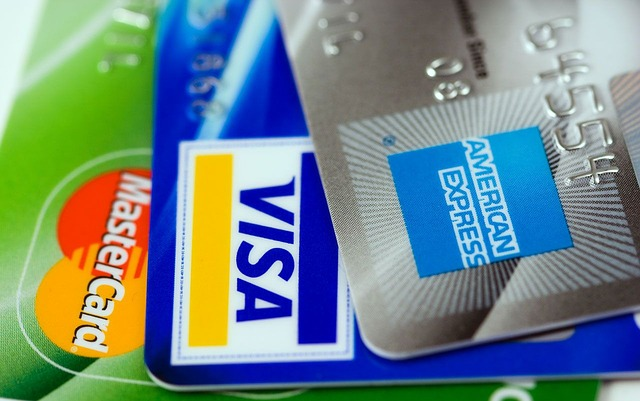
\includegraphics[scale=0.25]{CreditCards1}
\end{center}
\vfill
\pagebreak

\paragraph{Average Daily Balance Method} Different credit card companies calculate interest in different ways, all using the simple interest formula ($I=Prt$).  The difference lies in how $P$ is calculated; since the balance is constantly changing all month, they need a way to combine this all into a single principal.  The method we'll illustrate is called the \textit{average daily balance method}, which as the name suggests, takes the average of the balance on each day of the month.  Thus, if the balance was \$100 on the first 15 days of the month and \$200 on the last 15 days, the average daily balance will be \$150.

To find the average daily balance, add up the balance for each day and divide by the number of days.  In practice, we'll use a table to simplify the calculations by multiplying each different balance by the number of days that the card carried that balance.

\begin{example}[https://www.youtube.com/watch?v=ZUEQu_e2TqY]{Credit Card Charges}
Suppose your VISA card calculates interest using the average daily balance method, and the monthly interest rate is 1.5\% (notice that this means that the nominal annual rate is $1.5\% \times 12 = 18\%$, which is not at all unusually high for a credit card).  The itemized billing for the month of December is shown below.
\begin{center}
\begin{tabular}{l l l}
Detail & Date & Amount\\
\hline
Unpaid balance & December 1 & \$1500\\
Payment received & December 4 & \$300\\
Groceries & December 8 & \$125\\
Gas & December 15 & \$45\\
Wendy's & December 22 & \$8.50\\
Last day of billing period & December 31 &\\
Payment Due Date & January 7 &\\
\end{tabular}
\end{center}

\begin{enumerate}[(a)]
\item Find the average daily balance.

To do this, we'll build a table to keep track of the unpaid balance after each transaction, and how long that unpaid balance lasts.

\begin{center}
\begin{tabular}{l l}
Date & Unpaid Balance\\
\hline
December 1 & \$1500\\
December 4 & \$1200\\
December 8 & \$1325\\
December 15 & \$1370\\
December 22 & \$1378.50\\
\end{tabular}
\end{center}

Now calculate how many days each balance lasted and multiply the balance by the number of days it lasted; this lets us quickly add up the balance for each day so that we can find the average by dividing this by the number of days.
\begin{center}
\begin{tabular}{l l p{0.7in} p{1.5in}}
Date & Unpaid Balance & Number of Days & (Unpaid balance) $\times$ (Number of Days)\\
\hline
December 1 & \$1500 & 3 & \$4500\\
December 4 & \$1200 & 4 & \$4800\\
December 8 & \$1325 & 7 & \$9275\\
December 15 & \$1370 & 7 & \$9590\\
December 22 & \$1378.50 & 10 & \$12,406.50\\
\hline
\textbf{Total:} & & 31 & \$40,571.50
\end{tabular}
\end{center}

The average daily balance is then the sum of the daily balances divided by 31, the number of days in the billing period:
\[\dfrac{\$40,571.50}{31} = \$1308.76\]

\item Find the interest due for December.

Use the simple interest formula, noting that since the interest rate is given as a \textit{monthly} rate, $t=1$ since we're dealing with a single month:
\[I=Prt = (\$1308.76)(0.015)(1) = \$19.63\]

\item Find the total balance owed on the last day of the billing period.

This is the final balance plus the interest charges:
\[\$1378.50 + \$19.63 = \$1398.13\]

\item This credit card requires a \$15 minimum monthly payment or 1/36 of the amount due, whichever is higher.  What is the minimum monthly payment due by January 7?

Since 1.36 of the amount due is $\$1398.13/36 = \$38.84$, which is more than \$15, the minimum payment due will be \$38.84.
\end{enumerate}
\end{example}

\begin{try}[http://izzomath.com/103text/finance/example5.7/story.html]
Suppose your VISA card calculates interest using the average daily balance method, and the monthly interest rate is 1.8\%.  The itemized billing for the month of May is shown below.
\begin{center}
\begin{tabular}{l l l}
Detail & Date & Amount\\
\hline
Unpaid balance & May 1 & \$850\\
Payment received & May 5 & \$200\\
Groceries & May 7 & \$240\\
Gas & May 13 & \$33\\
Jewelry Store & May 25 & \$575\\
Last day of billing period & May 31 &\\
Payment Due Date & June 7 &\\
\end{tabular}
\end{center}

\begin{enumerate}[(a)]
\item Find the average daily balance.
\item Find the interest due for this month.
\item Find the total balance owed on the last day of the billing period.
\item This credit card requires a \$20 minimum payment or 1/24 of the amount due, whichever is higher.  What is the minimum monthly payment due for this month?
\end{enumerate}
\end{try}

We'll finish this discussion by taking another look at the trap of the minimum payment; we'll use the numbers from the preceding example.  A minimum payment of \$38.84 on a balance of \$1398.13 sounds pretty reasonable, but think about how long it would take to pay off this balance by only making the minimum payment each month (even without adding further charges), since the majority of the minimum payment will go toward interest.

Skipping over the details (this can be figured out using a simple spreadsheet), if you started with a balance of \$1398.13 and never added another charge, just making the minimum payment each month, it would take 123 months to pay it off, or over 10 years.  In doing so, you would end up paying a total of \$2571.46, or nearly twice what you owed.  The lesson is simple: pay off your credit card in full as much as possible, and don't live beyond your means in a way that requires the use of credit to get by.

\begin{exercises}
\ptwo{If you take out an auto loan of \$8500 at 5\% interest for 48 months, what will your monthly payment be?}
\ptwo{If you borrow \$13,000 to buy a boat, and the bank charges 7\% interest for 72 months, how much will you have to pay each month?}

\ptwo{Janine bought \$3000 of new furniture on credit.  Because her credit score isn't very good, the store is charging her a fairly high interest rate on the loan: 16\%.  If she agreed to pay off the furniture over two years, how much will she have to pay each month?}
\ptwo{Carly financed a new \$1200 television at 12\% for 48 months.  How much will she have to pay every month to pay this off?}

\ptwo{If you want to buy a car, and you can afford a monthly payment of \$175, how large of a loan can you get at 4.8\% interest over 60 months?}
\ptwo{Mary is going to finance new office equipment at a 2\% rate over a 4 year term.  If she can afford monthly payments of \$100, how much can she pay for the new office equipment?}

\ptwo{If you buy a \$33,000 car for \$1000 down and monthly payments of \$685 for 60 months, how much will you pay in total for the car?}
\ptwo{A car costs \$27,000, and you're offered a loan that requires \$800 down and a monthly payment of \$575 for 60 months, how much will you pay in interest?}

\ptwo{You want to buy a \$200,000 home.  You plan to pay 10\% as a down payment, and take out a 30-year loan at 4.75\% for the rest.  The bank requires 2 points at closing.
\begin{enumerate}[(a)]
\item How much is the loan amount going to be?
\item How much are the closing costs?
\item What will your monthly payments be?
\item How much will you pay in interest over the life of the loan?
\end{enumerate}}
\ptwo{You want to buy a \$375,000 home.  You plan to pay 20\% as a down payment, and take out a 30-year loan at 3.9\% for the rest.  The bank requires 1 point at closing.
\begin{enumerate}[(a)]
\item How much is the loan amount going to be?
\item How much are the closing costs?
\item What will your monthly payments be?
\item How much will you pay in interest over the life of the loan?
\end{enumerate}}

\ptwo{You can afford a \$900 per month mortgage payment.  You've found a 30-year loan at 5\% interest.
\begin{enumerate}[(a)]
\item How big of a loan can you afford?
\item How much total money will you pay the bank?
\item How much of that money is interest?
\end{enumerate}}
\ptwo{You can afford a \$17,900 per month mortgage payment.  You've found a 15-year loan at 3.85\% interest.
\begin{enumerate}[(a)]
\item How big of a loan can you afford?
\item How much total money will you pay the bank?
\item How much of that money is interest?
\end{enumerate}}

\pone{Suppose you take out a \$315,000 mortgage for 30 years at 4.5\% interest.
\begin{enumerate}[(a)]
\item Find the monthly payment on this mortgage.
\item Fill out the first two rows of the amortization schedule below.
\begin{center}
\begin{tabular}{|>{\centering\arraybackslash\hspace{0pt}}p{1.1in} | >{\centering\arraybackslash\hspace{0pt}}p{1.1in} | >{\centering\arraybackslash\hspace{0pt}}p{1.2in} | >{\centering\arraybackslash\hspace{0pt}}p{1in}|}
\hline
{\small Payment Number} & {\small Interest Payment} & {\small Principal Payment} & {\small Balance of Loan}\\
\hline
1 & & & \\
\hline
2 & & & \\
\hline
& & &
\end{tabular}
\end{center}
\end{enumerate}}

\pone{Suppose you take out a \$180,000 mortgage for 15 years at 3.7\% interest.
\begin{enumerate}[(a)]
\item Find the monthly payment on this mortgage.
\item Fill out the first two rows of the amortization schedule below.
\begin{center}
\begin{tabular}{|>{\centering\arraybackslash\hspace{0pt}}p{1.1in} | >{\centering\arraybackslash\hspace{0pt}}p{1.1in} | >{\centering\arraybackslash\hspace{0pt}}p{1.2in} | >{\centering\arraybackslash\hspace{0pt}}p{1in}|}
\hline
{\small Payment Number} & {\small Interest Payment} & {\small Principal Payment} & {\small Balance of Loan}\\
\hline
1 & & & \\
\hline
2 & & & \\
\hline
& & &
\end{tabular}
\end{center}
\end{enumerate}}

\ptwo{Suppose your VISA card calculates interest using the average daily balance method, and the monthly interest rate is 1.4\%.  The itemized billing for the month of April is shown below.\\

\begin{tabular}{l l l}
Detail & Date & Amount\\
\hline
Unpaid balance & April 1 & \$1100\\
Payment received & April 3 & \$500\\
New computer & April 11 & \$750\\
Books & April 15 & \$65\\
Mattress & April 28 & \$600\\
Last day of billing period & April 30 &\\
Payment Due Date & May 7 &\\
\end{tabular}

\begin{enumerate}[(a)]
\item Find the average daily balance.
\item Find the interest due for this month.
\item Find the total balance owed on the last day of the billing period.
\item This credit card requires a \$20 minimum payment or 1/36 of the amount due, whichever is higher.  What is the minimum monthly payment due for this month?
\end{enumerate}}
\ptwo{Suppose your MasterCard calculates interest using the average daily balance method, and the monthly interest rate is 2.1\%.  The itemized billing for the month of August is shown below.\\

\begin{tabular}{l l l}
Detail & Date & Amount\\
\hline
Unpaid balance & August 1 & \$300\\
Payment received & August 9 & \$100\\
Tuition & August 10 & \$4500\\
Textbooks & August 18 & \$350\\
Groceries & August 25 & \$180\\
Last day of billing period & August 31 &\\
Payment Due Date & September 7 &\\
\end{tabular}

\begin{enumerate}[(a)]
\item Find the average daily balance.
\item Find the interest due for this month.
\item Find the total balance owed on the last day of the billing period.
\item This credit card requires a \$15 minimum payment or 1/24 of the amount due, whichever is higher.  What is the minimum monthly payment due for this month?
\end{enumerate}}
\vfill
\pagebreak

\pone{\textbf{Project: Finding a Mortgage}

You and your family are looking to move and are shopping for a house.  Your job is to find a mortgage that you can afford.

You may choose your family size---you can be married with kids, married without kids, or single.  You may also pick anywhere in the country that you'd like to live, but you can only make the median income listed for the state you choose.  If you are married, you can assume that both you and your spouse are working and each are paid the median income for that state.

\begin{enumerate}
\item Decide where you want to live.  Do some research and find the median income for that state, and decide whether you are single or married, and whether or not you have children.
\item Search \href{http://www.realtor.com}{realtor.com} or a similar website to find a house that fits your family's needs.  Take note of the
\begin{itemize}
\item List price of the home.
\item Property taxes listed under the ``Property History'' tab.  If property taxes are not listed, estimate the annual property taxes as 2\% of the purchase price.
\end{itemize}
\item Estimate the down payment you can afford, and take note of the principal of the loan that you will need.
\item There are several options for financing your new home.  These include obtaining a fixed 15-year mortgage, a fixed 30-year mortgage or an adjustable rate mortgage.  Go to \href{http://www.ratesandpoints.com}{www.ratesandpoints.com} $\longrightarrow$ ``Mortgage Analyst.''  First click on ``Go'' for a 30 FRM (30-year fixed rate mortgage).  Pick two options---one with points and one without.  Repeat this process for 15 FRM.  Record these results in the table below.
\begin{center}
\begin{tabular}{|p{0.75in} | p{1.5in} | p{2in} | p{1.5in}|}
\hline
\textbf{Length of Mortgage} & \textbf{Interest Rate} & \textbf{Monthly Payment (PMT)} & \textbf{Total Cost of Mortgage = Total PMTs + Down Payment + Closing Cost}\\
\hline
& With 0 points & & \\
& Rate $= \line(1,0){30}$ & & \\
15 years & & & \\
& With $\line(1,0){30}$ points & & \\
& Rate $= \line(1,0){30}$ & & \\
\hline
& With 0 points & & \\
& Rate $= \line(1,0){30}$ & & \\
30 years & & & \\
& With $\line(1,0){30}$ points & & \\
& Rate $= \line(1,0){30}$ & & \\
\hline
\end{tabular}
\end{center}
Which option seems like the best?
\end{enumerate}}

\begin{minipage}{0.9\textwidth}
\begin{enumerate}
\setcounter{enumi}{4}
\item Complete the following steps to find if you can afford this home.
\begin{center}
\begin{tabular}{p{3.75in} p{3in}}
\textbf{Monthly Gross Income} &\\
\hspace{0.5in} Borrower's annual income & $\$ \line(1,0){150}$\\
& \\
\hspace{0.5in} Co-borrower's annual income & $+ \line(1,0){150}$\\
& \\
\hspace{0.5in} Total gross annual income & $\$ \line(1,0){150}$\\
\hspace{0.75in} Divide total gross income by 12 & \hspace{0.25in} $\div$ 12\\
& \\
\hspace{0.5in} Total monthly gross income & $\$ \line (1,0){150}$\\
\hspace{0.75in} Find 28\% of this & \hspace{0.25in} $\times 0.28$\\
& \\
\hspace{0.5in} \textbf{Allowable monthly housing cost} & $\$\line(1,0){150}$ (A)\\
& \\
\textbf{Monthly Taxes} &\\
\hspace{0.5in} Home purchase price & $\$ \line(1,0){150}$\\
& \\
\hspace{0.5in} Estimated taxes & $\$ \line(1,0){150}$\\
\hspace{0.75in} Divide taxes by 12 & \hspace{0.25in} $\div 12$\\
& \\
\hspace{0.5in} Monthly taxes & $\$ \line(1,0){150}$ (B)\\
& \\
\textbf{Monthly Housing Cost} & \\
\hspace{0.5in} Monthly mortgage payment & $\$ \line(1,0){150} \ +$\\
& \\
\hspace{0.5in} Estimated monthly taxes (B) & $\$ \line(1,0){150} \ +$\\
& \\
\hspace{0.5in} Condo or homeowner's fee (if applicable) & $\$ \line(1,0){150}$\\
& \\
\textbf{Total Monthly Housing Cost} & $= \$ \line(1,0){140}$ (C)
\end{tabular}
\end{center}
Compare (A) and (C).  Can you afford the house you want to buy?  If not, choose a less expensive house and redo this project.
\end{enumerate}
\end{minipage}

\end{exercises}